% Basic Category Theory
% Tom Leinster <Tom.Leinster@ed.ac.uk>
% 
% Copyright (c) Tom Leinster 2014-2016
% 
% Chapter 4: Representables
% 

\chapter{Representables}
\label{ch:rep}


A category is a world of objects, all looking at one another.  Each sees
the world from a different viewpoint.  

Consider, for instance, the category of topological spaces, and let us ask
how it looks when viewed from the one-point space $1$.  A map from $1$ to a
space $X$ is essentially the same thing as a point of $X$, so we might say
that $1$ `sees%
%
\index{functor!seeing@`seeing'}
%
points'.  Similarly, a map from $\reals$ to a space $X$
could reasonably be called a curve in $X$, and in this sense, $\reals$ sees
curves.

Now consider the category of groups.  A map from the infinite
cyclic group $\integers$%
%
\index{Z@$\integers$ (integers)!group@as group}
%
to a group $G$ amounts to an element of $G$.  (For given $g \in G$, there
is a unique homomorphism $\phi\from \integers \to G$ such that $\phi(1) =
g$.)  So, $\integers$ sees elements.  Similarly, if $p$ is a prime number
then the cyclic group $\integers/p\integers$ sees elements of order $1$ or
$p$.

Any ring homomorphism between fields is injective, so in the category of
fields,%
%
\index{field}
%
a map $K \to L$ is a way of realizing $L$ as an extension of $K$.  Hence
each field $K$ sees the extensions of itself.  If $K$ and $L$ are fields of
different characteristic then there are no homomorphisms between $K$ and
$L$, so the category of fields is the union of disjoint subcategories
$\Field_0$, $\Field_2$, $\Field_3$, $\Field_5$, \ldots\ consisting of the
fields of characteristics $0, 2, 3, 5$, \ldots.  Each field is blind to the
fields of different characteristic.

In the ordered set $(\reals, \mathord{\leq})$, the object $0$ sees whether
a number is nonnegative.  In other words, if $x$ is nonnegative then
there is one map $0 \to x$, and if not, there are none.

We can also ask the dual question: fixing an object of a category, what are
the maps \emph{into} it?  Let $S$ be the two-element set, for instance.
For an arbitrary set $X$, the maps from $X$ to $S$ correspond to the
subsets of $X$ (as we saw in Section~\ref{sec:Set-properties}).  Now give
$S$ the topology in which one of the singleton subsets is open but the
other is not.  For any topological space $X$, the continuous maps from $X$
into $S$ correspond to the \emph{open} subsets of $X$.

This chapter explores the theme of how each object sees and is seen by the
category in which it lives.  We are naturally led to the notion of
representable functor, which (after adjunctions) provides our second
approach to the idea of universal property.



\section{Definitions and examples}
\label{sec:rep-defns}


Fix an object $A$ of a category $\cat{A}$.  We will consider the totality
of maps out of $A$.  To each $B \in \cat{A}$, there is assigned the set
(or class) $\cat{A}(A, B)$ of maps from $A$ to $B$.  The content of the
following definition is that this assignation is functorial in $B$: any map
$B \to B'$ induces a function $\cat{A}(A, B) \to \cat{A}(A, B')$.

\begin{defn}  
\label{defn:co-rep}
Let $\cat{A}$ be a locally small category and $A \in \cat{A}$.  We define a
functor
\[
\h^A = \cat{A}(A, \dashbk)\from \cat{A} \to \Set%
%
\ntn{hom-out}
%
\]
as follows:
% 
\begin{itemize}
\item 
for objects $B \in \cat{A}$, put $\h^A(B) = \cat{A}(A, B)$;

\item 
for maps $B \toby{g} B'$ in $\cat{A}$, define
\[
\h^A(g) = \cat{A}(A, g)\from 
\cat{A}(A, B) \to \cat{A}(A, B')
\]
by 
\[
p 
\mapsto
g \of p
\]
for all $p\from A \to B$.
\end{itemize}
\end{defn}

\begin{remarks}
\begin{enumerate}[(b)]
\item 
Recall that `locally%
%
\index{locally small}%
\index{category!locally small}
%
small' means that each class $\cat{A}(A, B)$ is in fact a set.  This
hypothesis is clearly necessary in order for the definition to make sense.

\item 
Sometimes $\h^A(g)$ is written as $g \of \dashbk$%
%
\ntn{of-blank}
%
 or $g_*$.%
%
\ntn{lower-star}
%
All three forms, as well as $\cat{A}(A, g)$, are in use.
\end{enumerate}
\end{remarks}

\begin{defn}
Let $\cat{A}$ be a locally small category.  A functor $X\from \cat{A} \to
\Set$ is \demph{representable}%
%
\index{functor!representable}
%
if $X \iso \h^A$ for some $A \in \cat{A}$.
A \demph{representation}%
%
\index{representation!functor@of functor}
%
of $X$ is a choice of an object $A \in \cat{A}$ and an isomorphism between
$\h^A$ and $X$.
\end{defn}
% 
Representable functors are sometimes just called `representables'.  Only
set-valued%
%
\index{functor!set-valued}%
\index{set!valued functor@-valued functor}
%
functors (that is, functors with codomain $\Set$) can be representable.

\begin{example}        
\label{eg:co-reps-id-Set}
Consider $\h^1\from \Set \to \Set$, where $1$ is the one-element set.
Since a map from $1$ to a set $B$ amounts to an element of $B$, we have
\[
\h^1(B) \iso B
\]
for each $B \in \Set$.  It is easily verified that this isomorphism is
natural in $B$, so $\h^1$ is isomorphic to the identity functor $1_\Set$.
Hence $1_\Set$ is representable.
\end{example}

\begin{example}
\label{eg:co-reps-seeing}
All of the `seeing'%
%
\index{functor!seeing@`seeing'}
%
functors in the introduction to this chapter are representable.  The
forgetful%
%
\index{functor!forgetful!representable@is representable}
%
functor $\Tp \to \Set$ is isomorphic to $\h^1 = \Tp(1, \dashbk)$, and the
forgetful functor $\Grp \to \Set$ is isomorphic to $\Grp(\integers,
\dashbk)$.  For each prime $p$, there is a functor $U_p\from \Grp \to \Set$
defined on objects by
\[
U_p(G) = 
\{\text{elements of }G \text{ of order } 1 \text{ or } p \},
%
\index{group!order of element of}
%
\]
and as claimed above, $U_p \iso \Grp(\integers/p\integers, \dashbk)$
(Exercise~\ref{ex:cyclic-rep}).  Hence $U_p$ is representable.
\end{example}

\begin{example}
There is a functor $\ob\from \Cat \to \Set$ sending a small category to its
set% 
%
\index{object!set of category@-set of category}
% 
of objects.  (The category $\Cat$ was introduced in
Definition~\ref{defn:Cat}.) It is representable.  Indeed, consider the
terminal category $\One$ (with one object and only the identity map).  A
functor from $\One$ to a category $\cat{B}$ simply picks out an object of
$\cat{B}$.  Thus,
\[
\h^\One(\cat{B}) \iso \ob\cat{B}.
\]
Again, it is easily verified that this isomorphism is natural in $\cat{B}$;
hence $\ob \iso \Cat(\One, \dashbk)$.  It can be shown similarly that the
functor $\Cat \to \Set$ sending a small category to its set of maps is
representable (Exercise~\ref{ex:arrows-rep}).  
\end{example}

\begin{example}
Let $M$ be a monoid, regarded as a one-object%
%
\index{monoid!action of}
%
category.  Recall from Example~\ref{eg:functor-action} that a set-valued
functor on $M$ is just an $M$-set.  Since the category $M$ has only one
object, there is only one representable functor on it (up to isomorphism).
As an $M$-set, the unique representable is the so-called \demph{left
regular%
%
\index{representation!group or monoid@of group or monoid!regular}
%
representation} of $M$, that is, the underlying set of $M$ acted on by
multiplication on the left.
\end{example}

\begin{example}
Let $\Toph_*$%
%
\ntn{Toph-star}
%
be the category whose objects are topological spa\-ces equipped with a
basepoint and whose arrows are homotopy%
%
\index{homotopy}
%
classes of basepoint-preserving continuous maps.  Let $S^1 \in \Toph_*$%
%
\ntn{circle}
% 
be the circle.  Then for any object $X \in \Toph_*$, the maps $S^1 \to X$
in $\Toph_*$ are the elements of the fundamental%
%
\index{group!fundamental}
%
group $\pi_1(X)$.  Formally, this says that the composite functor
\[
\Toph_* \toby{\pi_1} \Grp \toby{U} \Set
\]
is isomorphic to $\Toph_*(S^1, \dashbk)$.  In particular, it is
representable.
\end{example}

\begin{example}
\label{eg:co-reps-tensor}
Fix a field $k$ and vector spaces $U$ and $V$ over $k$.  There is a
functor 
\[
\Bilin(U, V; \dashbk)\from \Vect_k \to \Set%
%
\index{map!bilinear}
%
\ntn{Bilin}
%
\]
whose value $\Bilin(U, V; W)$ at $W \in \Vect_k$ is the set of bilinear
maps $U \times V \to W$.  It can be shown that this functor is
representable; in other words, there is a space $T$ with the property that
\[
\Bilin(U, V; W) \iso \Vect_k(T, W)
\]
naturally in $W$.  This $T$ is the tensor%
%
\index{tensor product}
%
product $U \otimes V$, which we met just after the proof of
Lemma~\ref{lemma:tensor-unique}.
\end{example}

Adjunctions give rise to representable%
%
\index{functor!representable!adjoints@and adjoints}
%
functors in the following way.

\begin{lemma}   
\label{lemma:adj-to-rep}
Let $\hadjnli{\cat{A}}{\cat{B}}{F}{G}$ be locally small categories, and let
$A \in \cat{A}$.  Then the functor
\[
\cat{A}(A, G(\dashbk))\from \cat{B} \to \Set
\]
(that is, the composite $\cat{B} \toby{G} \cat{A} \toby{\h^A} \Set$) is
representable.  
\end{lemma}

\begin{pf}
We have
\[
\cat{A}(A, G(B)) \iso \cat{B}(F(A), B)
\]
for each $B \in \cat{B}$.  If we can show that this isomorphism is natural
in $B$, then we will have proved that $\cat{A}(A, G(\dashbk))$ is isomorphic
to $\h^{F(A)}$ and is therefore representable.  So, let $B \toby{q} B'$ be
a map in $\cat{B}$.  We must show that the square
\[
\xymatrix{
\cat{A}(A, G(B)) \ar[r] \ar[d]_{G(q) \of \dashbk}       &
\cat{B}(F(A), B) \ar[d]^{q \of \dashbk}        \\
\cat{A}(A, G(B')) \ar[r]        &
\cat{B}(F(A), B')
}
\]
commutes, where the horizontal arrows are the bijections provided by the
adjunction.  For $f \from A \to G(B)$, we have
\[
\xymatrix@C+3em{
f \ar@{|->}[r] \ar@{|->}[d]    &
\bar{f} \ar@{|->}[d]    \\
G(q) \of f \ar@{|->}[r]    &
*!<0mm,-1.4ex>+\txt{$q \of \bar{f}$\\
$\ovln{G(q) \of f}$,}
}
\]
so we must prove that $q \of \bar{f} = \ovln{G(q) \of f}$.  This follows
immediately from the naturality condition~\eqref{eq:adj-nat-a} in the
definition of adjunction (with $g = \bar{f}$). 
\end{pf}

You would not expect a randomly-chosen functor into $\Set$ to be
rep\-re\-sen\-table.  In some sense, rather few functors are.  However,
forgetful%
%
\index{functor!forgetful!representable@is representable|(}
%
functors do tend to be representable:
% 
\begin{propn}   
\label{propn:ladj-rep}
\hspace*{-2.5pt}Any set-valued functor with a left adjoint is representable.
\end{propn}

\begin{pf}
Let $G\from \cat{A} \to \Set$ be a functor with a left adjoint $F$.  Write
$1$ for the one-point set.  Then
\[
G(A) \iso \Set(1, G(A))
\]
naturally in $A \in \cat{A}$
(by Example~\ref{eg:co-reps-id-Set}), that is, $G \iso
\Set(1, G(\dashbk))$.  So by Lemma~\ref{lemma:adj-to-rep}, $G$ is
representable; indeed, $G \iso \h^{F(1)}$.  
\end{pf}

\begin{example}        
Several of the examples of representables mentioned above arise as in
Proposition~\ref{propn:ladj-rep}.  For instance, $U \from \Tp \to \Set$
has a left adjoint $D$%
%
\index{topological space!discrete}
%
(Example~\ref{eg:adjn:spaces}), and $D(1) \iso 1$, so we recover the result
that $U \iso \h^1$.  Similarly, Exercise~\ref{ex:cdoi} asked you to
construct a left adjoint $D$%
% 
\index{category!discrete}
%
to the objects functor $\ob\from \Cat \to \Set$.  This functor $D$
satisfies $D(1) \iso \One$, proving again that $\ob \iso \h^\One$.
\end{example}

\begin{example}
The forgetful functor $U\from \Vect_k \to \Set$ is representable,\linebreak
since it has a left adjoint.%
%
\index{vector space!free}
%
Indeed, if $F$ denotes the left adjoint then $F(1)$ is the $1$-dimensional
vector space $k$, so $U \iso \h^k$.  This is also easy to see directly: a
map from $k$ to a vector space $V$ is uniquely determined by the image of
$1$, which can be any element of $V$; hence $\Vect_k(k, V) \iso U(V)$
naturally in $V$.
\end{example}

\begin{example}
\label{eg:ladj-rep-ring}
Examples~\ref{egs:adjns-alg} began with the declaration that forgetful%
%
\index{functor!forgetful!left adjoint to}
%
functors between categories of algebraic structures usually have left
adjoints.  Take the category $\CRing$ of commutative rings%
%
\index{ring!free}
%
and the forgetful functor $U\from \CRing \to \Set$.  This general principle
suggests that $U$ has a left adjoint, and Proposition~\ref{propn:ladj-rep}
then tells us that $U$ is representable.

Let us see how this works explicitly.  Given a set $S$, let $\integers[S]$
be the ring of polynomials%
%
\index{ring!polynomial}
%
over $\integers$ in commuting variables $x_s$ ($s \in S$).  (This was
called $F(S)$ in Example~\ref{egs:free-functors}\bref{eg:free-ring}.)  Then
$S \mapsto \integers[S]$ defines a functor $\Set \to \CRing$, and this is
left adjoint to $U$.  Hence $U \iso \h^{\integers[x]}$.  Again, this
can be verified directly: for any ring $R$, the maps $\integers[x] \to R$
correspond one-to-one with the elements of $R$ (Exercises~\ref{ex:Zx}
and~\ref{ex:free-ring-one-gen}).
%
\index{functor!forgetful!representable@is representable|)}
\end{example}

We have defined, for each object $A$ of our category $\cat{A}$, a functor
$\h^A \in \ftrcat{\cat{A}}{\Set}$.  This describes how $A$ sees the world.
As $A$ varies, the view varies.  On the other hand, it is always the same
world being seen, so the different views from different objects are somehow
related.  (Compare aerial%
%
\index{aerial photography}
%
photos taken from a moving aeroplane, which agree well enough on their
overlaps that they can be patched together to make one big picture.)  So
the family $\bigl(\h^A\bigr)_{A \in \cat{A}}$ of `views' has some
consistency to it.  What this means is that whenever there is a map between
objects $A$ and $A'$, there is also a map between $\h^A$ and $\h^{A'}$.

Precisely, a map $A' \toby{f} A$ induces a natural transformation
\[
\xymatrix@C+1em{
\cat{A} \rtwocell<4>^{\h^A}_{\h^{A'}}{\hspace{.5em}\h^f} &\Set,
}%
%
\ntn{hom-out-map}
%
\]
whose $B$-component (for $B \in \cat{A}$) is the function  
\[
\begin{array}{ccc}
\h^A(B) = \cat{A}(A, B)  &\to            &\h^{A'}(B) = \cat{A}(A', B)     \\
p                       &\mapsto        &p \of f.
\end{array}
\]
Again, $\h^f$
goes by a variety of other names: $\cat{A}(f, \dashbk)$,%
%
\ntn{hom-out-map-blank}
%
$f^*$,%
%
\ntn{upper-star}
%
and $\dashbk \of f$.%
%
\ntn{blank-of}
%

Note the reversal of direction!  Each functor $\h^A$ is covariant, but they
come together to form a \emph{contravariant} functor, as in the following
definition. 

\begin{defn}
Let $\cat{A}$ be a locally small category.  The functor
\[
\h^\bl\from \cat{A}^\op \to \ftrcat{\cat{A}}{\Set}%
%
\ntn{hom-out-blank}
%
\]
is defined on objects $A$ by $\h^\bl(A) = \h^A$ and on maps $f$ by $\h^\bl(f)
= \h^f$. 
\end{defn}

The symbol $\bl$ is another type of blank, like $\dashbk$.  

All of the definitions presented so far in this chapter can be dualized.
At the formal level, this is trivial: reverse all the arrows, so that every
$\cat{A}$ becomes an $\cat{A}^\op$ and vice versa.  But in our usual
examples, the flavour is different.  We are no longer asking what objects
\emph{see}, but how they are \emph{seen}.

Let us first dualize Definition~\ref{defn:co-rep}.

\begin{defn}
Let $\cat{A}$ be a locally small category and $A \in \cat{A}$.  We define a
functor
\[
\h_A = \cat{A}(\dashbk, A)\from \cat{A}^\op \to \Set%
%
\ntn{hom-in}
%
\]
as follows:
% 
\begin{itemize}
\item 
for objects $B \in \cat{A}$, put $\h_A(B) = \cat{A}(B, A)$;

\item 
for maps $B' \toby{g} B$ in $\cat{A}$, define
\[
\h_A(g) = \cat{A}(g, A) = g^* = \dashbk \of g\from 
\cat{A}(B, A) \to \cat{A}(B', A)
\]
by 
\[
p 
\mapsto
p \of g
\]
for all $p\from B \to A$.
\end{itemize}
\end{defn}

If you know about dual vector spaces, this construction will seem familiar.
In particular, you will not be surprised that a map $B' \to B$ induces a
map in the opposite direction, $\h_A(B) \to \h_A(B')$.

We now define representability for \emph{contravariant} set-valued
functors.  Stri\-ctly speaking, this is unnecessary, as a contravariant
functor on $\cat{A}$ is a covariant functor on $\cat{A}^\op$, and we
already know what it means for a covariant set-valued functor to be
representable.  But it is useful to have a direct definition.

\begin{defn}
Let $\cat{A}$ be a locally small category.  A functor $X\from \cat{A}^\op \to
\Set$ is \demph{representable}%
%
\index{functor!representable}
%
if $X \iso \h_A$ for some $A \in \cat{A}$.  A \demph{representation}%
%
\index{representation!functor@of functor}
%
of $X$ is a choice of an object $A \in \cat{A}$ and an isomorphism between
$\h_A$ and $X$.
\end{defn}

\begin{example}        
There is a functor
\[
\pset\from \Set^\op \to \Set%
%
\ntn{power-set-ftr}
%
\]
sending each set $B$ to its power%
%
\index{power!set}
%
set $\pset(B)$, and defined on maps $g\from B' \to B$ by $(\pset(g))(U) =
g^{-1}U$ for all $U \in \pset(B)$.  (Here $g^{-1}U$ denotes the inverse%
%
\index{inverse!image}
%
image or preimage of $U$ under $g$, defined by $g^{-1} U = \{ x' \in B'
\such g(x') \in U \}$.)  As we saw in Section~\ref{sec:Set-properties}, a
subset amounts to a map into the two-point%
%
\index{set!two-element}
%
set $2$.  Precisely put, $\pset \iso \h_2$.
\end{example}

\begin{example}
\label{eg:contra-rep-sier}
Similarly, there is a functor
\[
\oset\from\Tp^\op \to \Set%
%
\ntn{oset-ftr}
%
\index{topological space!open subset of}%
\index{open subset}%
\index{set!open}
%
\]
defined on objects $B$ by taking $\oset(B)$ to be the set of open subsets
of $B$.  If $S$ denotes the two-point%
%
\index{topological space!two-point}
%
topological space in which exactly one of the two singleton subsets is
open, then continuous maps from a space $B$ into $S$ correspond naturally
to open subsets of $B$ (Exercise~\ref{ex:sierpinski-space}).  Hence $\oset
\iso \h_S$, and $\oset$ is representable.
\end{example}

\begin{example}
In Example~\ref{eg:contra-fn-spaces}, we defined a functor $C\from \Tp^\op
\to \Ring$, assigning to each space the ring%
%
\index{ring!functions@of functions}
%
of continuous real-valued functions%
%
\index{topological space!functions on}
%
on it.  The composite functor
\[
\Tp^\op \toby{C} \Ring \toby{U} \Set
\]
is representable, since by definition, $U(C(X)) = \Tp(X, \reals)$ for
topological spaces $X$.
\end{example}

Previously, we assembled the covariant representables $\bigl( \h^A
\bigr)_{A \in \cat{A}}$ into one big functor $\h^\bl$.  We now do the same
for the contravariant representables $\bigl( \h_A \bigr)_{A \in \cat{A}}$.
Any map $A \toby{f} A'$ in $\cat{A}$ induces a natural transformation
\[
\xymatrix@C+1em{
\cat{A}^\op \rtwocell<4>^{\h_A}_{\h_{A'}}{\hspace{.3em}\h_f} &\Set%
%
\ntn{hom-in-map}
%
}
\]
(also called $\cat{A}(\dashbk, f)$,%
%
\ntn{hom-in-map-blank}
%
$f_*$%
%
\ntn{lower-star-bis}
%
or $f \of \dashbk$),%
%
\ntn{of-blank-bis}
%
whose component at an object $B \in \cat{A}$ is
\[
\begin{array}{ccc}
\h_A(B) = \cat{A}(B, A)  &\to               &
\h_{A'}(B) = \cat{A}(B, A')     \\
p                       &\mapsto            &
f \of p.
\end{array}
\]

\begin{defn}    
\label{defn:yon-emb}
Let $\cat{A}$ be a locally small category.  The \demph{Yoneda%
%
\index{Yoneda embedding}
%
embedding} of $\cat{A}$ is the functor
\[
\h_\bl\from \cat{A} \to \ftrcat{\cat{A}^\op}{\Set}%
%
\ntn{hom-in-blank}
%
\]
defined on objects $A$ by $\h_\bl(A) = \h_A$ and on maps $f$ by $\h_\bl(f) =
\h_f$. 
\end{defn}

Here is a summary of the definitions so far.
% 
\begin{center}
\begin{tabular}{ll}
\ \\[-2ex]
For each $A \in \cat{A}$, we have a functor     &
$\cat{A} \toby{\h^A} \Set$. \\
Putting them all together gives a functor       &
$\cat{A}^\op \toby{\h^\bl} \ftrcat{\cat{A}}{\Set}$.
\vspace*{2ex}\\
For each $A \in \cat{A}$, we have a functor     &
$\cat{A}^\op \toby{\h_A} \Set$. \\
Putting them all together gives a functor       &
$\cat{A} \toby{\h_\bl} \ftrcat{\cat{A}^\op}{\Set}$.\\[-2ex]
\ 
\end{tabular}%
\end{center}
% 
The second pair of functors is the dual of the first.  Both involve
contravariance;%
%
\index{functor!contravariant}%
\index{contravariant}
%
it cannot be avoided.

In the theory of representable functors, it does not make much difference
whether we work with the first or the second pair.  Any theorem that we
prove about one dualizes to give a theorem about the other.  We choose to
work with the second pair, the $\h_A$s and $\h_\bl$.  In a sense to be
explained, $\h_\bl$ `embeds' $\cat{A}$ into $\ftrcat{\cat{A}^\op}{\Set}$.
This can be useful, because the category $\ftrcat{\cat{A}^\op}{\Set}$ has
some good properties that $\cat{A}$ might not have.

Exercise~\ref{ex:yoneda-conservative} asks you to prove that $\h_\bl$ is
injective on isomorphism classes of objects.  It is strongly recommended
that you do it before reading on, as it encapsulates the key ideas of the
rest of this chapter.

There is one more functor to define.  It unifies the first and second pairs
of functors shown above.

\begin{defn}
Let $\cat{A}$ be a locally small category.  The functor
\[
\Hom_\cat{A}\from \cat{A}^\op \times \cat{A} \to \Set%
%
\index{hom-set}
%
\ntn{Hom-functor}
%
\]
is defined by
\[
\xymatrix{
(A, B) \ar@<1ex>[d]^g    &
\mapsto \ar@{}[d]|*+{\mapsto}       &
\cat{A}(A, B) \ar[d]^{g \of \dashbk \of f}      \\
(A', B') \ar@<1ex>[u]^f  &
\mapsto &
\cat{A}(A', B').
}
\]
In other words, $\Hom_\cat{A}(A, B) = \cat{A}(A, B)$ and $(\Hom_\cat{A}(f,
g))(p) = g \of p \of f$, whenever $A' \toby{f} A \toby{p} B \toby{g} B'$.
\end{defn}

\begin{remarks}         
\label{rmks:global-hom}
\begin{enumerate}[(b)]
\item 
The existence of the functor $\Hom_\cat{A}$ is something like the fact that for
a metric%
%
\index{metric space}
%
space $(X, d)$, the metric is itself a continuous map $d\from X \times X
\to \reals$.  (If we take two points and move each one slightly, the
distance between them changes only slightly.)

\item 
In terms of Exercise~\ref{ex:ftr-on-product}, $\Hom_{\cat{A}}$ is the
functor $\cat{A}^\op \times \cat{A} \to \Set$ corresponding to the families
of functors $\bigl( \h^A \bigr)_{A \in \cat{A}}$ and $\bigl( \h_B \bigr)_{B
  \in \cat{A}}$.

\item   
\label{rmks:global-hom:cc}
In Example~\ref{eg:adjn:cc}, we saw that for any set $B$, there is an
adjunction $(\dashbk \times B) \ladj (\dashbk)^B$ of functors $\Set \to
\Set$.  Similarly, for any category $\cat{B}$, there is an adjunction
$(\dashbk \times \cat{B}) \ladj \ftrcat{\cat{B}}{\dashbk}$ of functors
$\CAT \to \CAT$; in other words, there is a canonical bijection
\[
\CAT(\cat{A} \times \cat{B}, \cat{C})
\iso
\CAT(\cat{A}, \ftrcat{\cat{B}}{\cat{C}})
\]
for $\cat{A}, \cat{B}, \cat{C} \in \CAT$.  Under this bijection, the functors
\[
\Hom_\cat{A}\from \cat{A}^\op \times \cat{A} \to \Set,
\qquad
\h^\bl\from \cat{A}^\op \to \ftrcat{\cat{A}}{\Set}
\]
correspond to one another.  Thus, $\Hom_\cat{A}$ carries the same
information as $\h^\bl$ (or $\h_\bl$), presented slightly differently.
\end{enumerate}
\end{remarks}

\begin{remark}  
\label{rmk:adj-nat}
We can now explain the naturality%
%
\index{adjunction!naturality axiom for}
%
in the definition of adjunction (Definition~\ref{defn:adjn}).  Take
categories and functors $\oppairi{\cat{A}}{\cat{B}}{F}{G}$.  They give rise
to functors
\[
\xymatrix{
\cat{A}^\op \times \cat{B} \ar[r]^-{1\times G} \ar[d]_{F^\op \times 1} &
\cat{A}^\op \times \cat{A} \ar[d]^{\Hom_\cat{A}}        \\
\cat{B}^\op \times \cat{B} \ar[r]_-{\Hom_\cat{B}} &
\Set.
}
\]
The composite functor $\searrows$ sends $(A, B)$ to $\cat{B}(F(A), B)$; it
can be written as $\cat{B}(F(\dashbk), \dashbk)$.  The composite
$\esarrows$ sends $(A, B)$ to $\cat{A}(A, G(B))$.
Exercise~\ref{ex:adj-nat} asks you to show that these two functors
\[
\cat{B}(F(\dashbk), \dashbk), 
\ 
\cat{A}(\dashbk, G(\dashbk))
\from
\cat{A}^\op \times \cat{B} \to \Set
\]
are naturally isomorphic if and only if $F$ and $G$ are adjoint.  This
justifies the claim in Remark~\ref{rmks:adjts}\bref{rmk:adjts:nat}: the
naturality requirements~\eqref{eq:adj-nat-a} and~\eqref{eq:adj-nat-b} in
the definition of adjunction simply assert that two particular functors
are naturally isomorphic.
\end{remark}

Objects of an arbitrary category do not have elements in any obvious sense.
However, \emph{sets} certainly have elements, and we have observed that an
element of a set $A$ is the same thing as a map $1 \to A$.  This inspires
the following definition.

\begin{defn}    
\label{defn:gen-elt}
Let $A$ be an object of a category.  A \demph{generalized%
%
\index{element!generalized}
%
element} of $A$ is a map with codomain $A$.  A map $S \to A$ is a
generalized element of $A$ of \demph{shape%
%
\index{shape!generalized element@of generalized element}
%
$S$}.
\end{defn}

`Generalized element' is nothing more than a synonym of `map', but
sometimes it is useful to think of maps as generalized elements.

For example, when $A$ is a set, a generalized element of $A$ of shape $1$
is an ordinary element of $A$, and a generalized element of $A$ of shape
$\nat$ is a sequence%
%
\index{sequence}
%
in $A$.  In the category of topological spaces, the generalized elements of
shape $1$ (the one-point space) are the points, and the generalized
elements of shape $S^1$ (the circle) are, by definition, loops.%
%
\index{loop|(}
%
As this suggests, in categories of geometric objects, we might equally well
say `figures of shape $S$'.

In algebra,%
%
\index{algebra}
%
we are often interested in solutions to equations such as $x^2 + y^2 = 1$.
Perhaps we begin by being particularly interested in solutions in
$\rationals$, but then realize that in order to study rational solutions,
it will be helpful to study solutions in other rings first.  (This is often
a fruitful strategy.)  Given a ring $A$, a pair $(a, b) \in A \times A$
satisfying $a^2 + b^2 = 1$ amounts to a homomorphism of rings
\[
\integers[x, y]/(x^2 + y^2 - 1) \to A.
%
\index{algebraic geometry}
%
\]
Thus, the solutions to our equation (in any ring) can be seen as the
generalized elements of shape $ \integers[x, y]/(x^2 + y^2 - 1)$.

For an object $S$ of a category $\cat{A}$, the functor
\[
\h^S\from \cat{A} \to \Set
\]
sends an object to its set of generalized elements of shape $S$.  The
functoriality tells us that any map $A \to B$ in $\cat{A}$ transforms
$S$-elements of $A$ into $S$-elements of $B$.  For example, taking $\cat{A}
= \Tp$ and $S = S^1$, any continuous map $A \to B$ transforms loops in $A$
into loops in $B$.%
%
\index{loop|)}
%


\exs


\begin{question}
Find three examples of representable functors not mentioned above.
\end{question}


\begin{question}        
\label{ex:yoneda-conservative}
Let $\cat{A}$ be a locally small category, and let $A, A' \in \cat{A}$ with
$\h_A \iso \h_{A'}$.  Prove directly that $A \iso A'$.
\end{question}


\begin{question}        
\label{ex:cyclic-rep}
Let $p$ be a prime number.  Show that the functor $U_p\from \Grp \to \Set$
defined in Example~\ref{eg:co-reps-seeing} is isomorphic to
$\Grp(\integers/p\integers, \dashbk)$.  (To check that there is an
isomorphism of functors~-- that is, a \emph{natural} isomorphism~-- you
will first need to define $U_p$ on maps.  There is only one sensible way to
do this.)
\end{question}


\begin{question}        
\label{ex:free-ring-one-gen}
Using the result of Exercise~\ref{ex:Zx}\bref{part:Zx-main}, prove that the
forgetful functor $\CRing \to \Set$ is isomorphic to $\CRing(\integers[x],
\dashbk)$, as in Example~\ref{eg:ladj-rep-ring}.
\end{question}


\begin{question}        
\label{ex:sierpinski-space}
The \demph{Sierpi\'nski%
%
\index{Sierpi\'nski space}
%
space} is the two-point topological space $S$ in
which one of the singleton subsets is open but the other is not.  Prove
that for any topological space $X$, there is a canonical bijection between
the open subsets of $X$ and the continuous maps $X \to S$.  Use this to
show that the functor $\oset\from \Tp^\op \to \Set$ of
Example~\ref{eg:contra-rep-sier} is represented by $S$.
\end{question}


\begin{question}        
\label{ex:arrows-rep}
Let $M \from \Cat \to \Set$ be the functor that sends a small category
$\cat{A}$ to the set of all maps in $\cat{A}$.  Prove that $M$ is
representable.
\end{question}


\begin{question}        
\label{ex:adj-nat}
Take locally small categories $\cat{A}$ and $\cat{B}$, and functors
$\oppairi{\cat{A}}{\cat{B}}{F}{G}$.  Show that $F$ is left adjoint to $G$
if and only if the two functors 
\[
\cat{B}(F(\dashbk), \dashbk), 
\ 
\cat{A}(\dashbk, G(\dashbk))
\from
\cat{A}^\op \times \cat{B} \to \Set
\]
of Remark~\ref{rmk:adj-nat} are naturally isomorphic.  (Hint: this
  is made easier by using either Exercise~\ref{ex:nat-iso-on-product} or
  Exercise~\ref{ex:adj-nat-in-one}.)
\end{question}



\section{The Yoneda lemma}


What do representables see?

Recall from Definition~\ref{defn:presheaf} that functors $\cat{A}^\op \to
\Set$ are sometimes called `presheaves' on $\cat{A}$.  So for each $A \in
\cat{A}$ we have a representable presheaf $\h_A$, and we are asking how the
rest of the presheaf category $\pshf{\cat{A}}$ looks from the viewpoint of
$\h_A$.  In other words, if $X$ is another presheaf, what are the maps
$\h_A \to X$?

Newcomers to category theory commonly find that the material presented in
this section is where they first get stuck.  Typically, the core of the
difficulty is in understanding the question just asked.  Let us ask it
again. 

We start by fixing a locally small category $\cat{A}$.  We then take an
object $A \in \cat{A}$ and a functor $X\from \cat{A}^\op \to \Set$.  The
object $A$ gives rise to another functor $\h_A = \cat{A}(\dashbk, A)\from
\cat{A}^\op \to \Set$.  The question is: what are the maps $\h_A \to X$?
Since $\h_A$ and $X$ are both objects of the presheaf category
$\pshf{\cat{A}}$, the `maps' concerned are maps in $\pshf{\cat{A}}$.  So,
we are asking what natural transformations
% 
\begin{equation}        
\label{eq:yoneda-transf}
\begin{array}{c}
\xymatrix{
\cat{A}^\op \rtwocell^{\h_A}_{X} &\Set
}
\end{array}
\end{equation}
% 
there are.  The set of such natural transformations is called
\[
\pshf{\cat{A}}(\h_A, X).
\]
(This is a special case of the notation $\cat{B}(B, B')$ for the set of
maps $B \to B'$ in a category $\cat{B}$.  Here, $\cat{B} = \pshf{\cat{A}}$,
$B = \h_A$, and $B' = X$.)  We want to know what this set is.

There is an informal principle%
%
\index{uniqueness!constructions@of constructions|(}
%
of general category theory that allows us to
guess the answer.  Look back at
Remarks~\ref{rmks:defn-cat}\bref{rmk:defn-cat:loosely},
\ref{rmks:defn-ftr}\bref{rmk:defn-ftr:loosely}
and~\ref{rmks:defn-nt}\bref{rmk:defn-nt:loosely} on the definitions of
category, functor and natural transformation.  Each remark is of the form
`from input of one type, it is possible to construct exactly one output of
another type'.  For example, in
Remark~\ref{rmks:defn-cat}\bref{rmk:defn-cat:loosely}, the input is a
sequence of maps $A_0 \toby{f_1} \cdots \toby{f_n} A_n$, the output is a
map $A_0 \to A_n$, and the statement is that no matter what we do with the
input data $f_1, \ldots, f_n$, there is only one map $A_0 \to A_n$ that we
can construct.

Let us apply this principle to our question.  We have just seen how, given
as input an object $A \in \cat{A}$ and a presheaf $X$ on $\cat{A}$, we can
construct a set, namely, $\pshf{\cat{A}}(\h_A, X)$.  Are there any other
ways to construct a set from the same input data $(A, X)$?  Yes: simply
take the set $X(A)$!  The informal principle suggests that these two sets
are the same:
% 
\begin{equation}        
\label{eq:yoneda-pre}
\pshf{\cat{A}}(\h_A, X) \iso X(A)
\end{equation}
% 
for all $A \in \cat{A}$ and $X \in \pshf{\cat{A}}$.  This turns out to be
true; and that is the Yoneda lemma.%
%
\index{uniqueness!constructions@of constructions|)}
%
  
Informally, then, the Yoneda lemma says that for any $A \in \cat{A}$ and
presheaf $X$ on $\cat{A}$:
% 
\begin{slogan}
A natural transformation $\h_A \to X$ is an element of $X(A)$.
\end{slogan}
% 
Here is the formal statement.  The proof follows shortly.

\begin{thm}[Yoneda]   
\label{thm:yoneda}
%
\index{Yoneda lemma}
%
Let $\cat{A}$ be a locally small category.  Then
% 
\begin{equation}        
\label{eq:yoneda}
\pshf{\cat{A}}(\h_A, X)
\iso
X(A)
\end{equation}
% 
naturally in $A \in \cat{A}$ and $X \in \pshf{\cat{A}}$.  
\end{thm}

This is exactly what was stated in~\eqref{eq:yoneda-pre}, except that the
word `naturally' has appeared.  Recall from Definition~\ref{defn:nat-in}
that for functors $F, G\from \cat{C} \to \cat{D}$, the phrase `$F(C) \iso
G(C)$ naturally in $C$' means that there is a natural isomorphism $F \iso
G$.  So the use of this phrase in the Yoneda lemma suggests that each side
of~\eqref{eq:yoneda} is functorial in both $A$ and $X$.  This means, for
instance, that a map $X \to X'$ must induce a map
\[
\pshf{\cat{A}}(\h_A, X) 
\to
\pshf{\cat{A}}(\h_A, X'),
\]
and that not only does the isomorphism~\eqref{eq:yoneda} hold for
\emph{every} $A$ and $X$, but also, the isomorphisms can be chosen in a way
that is compatible with these induced maps.  Precisely, the Yoneda lemma
states that the composite functor
\[
\xymatrix@R=0em{
\cat{A}^\op \times \pshf{\cat{A}}  \ar[r]^-{\h_\bl^\op \times 1} &
{\pshf{\cat{A}}}^\op \times \pshf{\cat{A}} 
\ar[r]^-{\Hom_{\pshf{\cat{A}}}} &
\Set    \\
(A, X) \ar@{}[r]|(.43)*+{\longmapsto} &
(\h_A, X) \ar@{}[r]|(.55)*+{\longmapsto} &
\pshf{\cat{A}}(\h_A, X)
}
\]
is naturally isomorphic to the evaluation%
%
\index{evaluation}
%
 functor
\[
\begin{array}{ccc}
\cat{A}^\op \times \pshf{\cat{A}}       &\to            &\Set   \\
(A, X)                                  &\mapsto        &X(A).
\end{array}
\]

If the Yoneda lemma were false then the world would look much more complex.
For take a presheaf $X\from \cat{A}^\op \to \Set$, and define a new
presheaf $X'$ by
\[
X' = \pshf{\cat{A}}(\h_\bl, X)
\from 
\cat{A}^\op \to \Set,
\]
that is, $X'(A) = \pshf{\cat{A}}(\h_A, X)$ for all $A \in \cat{A}$.  Yoneda
tells us that $X'(A) \iso X(A)$ naturally in $A$; in other words, $X' \iso
X$.  If Yoneda were false then starting from a single presheaf $X$, we
could build an infinite sequence $X, X', X'', \ldots$ of new presheaves,
potentially all different.  But in reality, the situation is very simple:
they are all the same.

The proof of the Yoneda lemma is the longest proof so far.  Nevertheless,
there is essentially only one way to proceed at each stage.  If you suspect
that you are one of those newcomers to category theory for whom the Yoneda
lemma presents the first serious challenge, an excellent exercise is to
work out the proof before reading it.  No ingenuity is required, only an
understanding of all the terms in the statement.

\begin{pfof}{the Yoneda lemma}
We have to define, for each $A$ and $X$, a bijection between the sets
$\pshf{\cat{A}}(\h_A, X)$ and $X(A)$.  We then have to show that our bijection
is natural in $A$ and $X$.

First, fix $A \in \cat{A}$ and $X \in \pshf{\cat{A}}$.  We define functions
% 
\begin{equation}        
\label{eq:yoneda-fns}
\oppair{\pshf{\cat{A}}(\h_A, X)}{X(A)}{\yel{\blank}}{\ynt{\blank}}
\end{equation}
% 
and show that they are mutually inverse.  So we have to do four things: define
the function $\yel{\blank}$, define the function $\ynt{\blank}$, show that
$\yel{\ynt{\blank}}$ is the identity, and show that $\ynt{\yel{\blank}}$ is
the identity.
% 
\begin{itemize}
\item 
Given $\alpha\from \h_A \to X$, define $\yel{\alpha} \in X(A)$ by
$\yel{\alpha} = \alpha_A(1_A)$.  (How else could we possibly define it?)

\item 
Let $x \in X(A)$.  We have to define a natural transformation $\ynt{x}\from
\h_A \to X$.  That is, we have to define for each $B \in \cat{A}$ a
function
\[
\ynt{x}_B\from \h_A(B) = \cat{A}(B, A) \to X(B)
\]
and show that the family $\ynt{x} = (\ynt{x}_B)_{B \in \cat{A}}$ satisfies
naturality.  

Given $B \in \cat{A}$ and $f \in \cat{A}(B, A)$, define
\[
\ynt{x}_B(f) = (X(f))(x) \in X(B).
\]
(How else could we possibly define it?)  This makes sense, since $X(f)$ is a
map $X(A) \to X(B)$.  To prove naturality, we must show that for any map
$B' \toby{g} B$ in $\cat{A}$, the square
\[
\xymatrix@C+4em@R+1ex{
\cat{A}(B, A) \ar[r]^{\h_A(g)\: =\: \dashbk\of g} \ar[d]_{\ynt{x}_B}        &
\cat{A}(B', A) \ar[d]^{\ynt{x}_{B'}} \\
X(B) \ar[r]_{X(g)}        &
X(B')
}
\]
commutes.  To reduce clutter, let us write $X(g)$ as $Xg$, and so on.  Now
for all $f \in \cat{A}(B, A)$, we have
\[
\xymatrix@C+3em{
f \ar@{|->}[r] \ar@{|->}[d]    &
f \of g \ar@{|->}[d]    \\
(Xf)(x) \ar@{|->}[r]    &
*!<0mm,-1.4ex>+\txt{$(X(f\of g))(x)$\\
$(Xg)((Xf)(x))$,}
}
\]
and $X(f \of g) = (Xg) \of (Xf)$ by functoriality, so the square does commute.

\item 
Given $x \in X(A)$, we have to show that $\yel{\ynt{x}} = x$, and indeed,
\[
\yel{\ynt{x}}
=
\ynt{x}_A(1_A)
=
(X 1_A)(x)
=
1_{X(A)}(x)
=
x.
\]

\item 
Given $\alpha\from \h_A \to X$, we have to show that $\ynt{\yel{\alpha}} =
\alpha$.  Two natural transformations are equal if and only if all their
components are equal; so, we have to show that
$\Bigl(\ynt{\yel{\alpha}}\Bigr)_B = \alpha_B$ for all $B \in \cat{A}$.
Each side of this equation is a function from $\h_A(B) = \cat{A}(B, A)$ to
$X(B)$, and two functions are equal if and only if they take equal values
at every element of the domain; so, we have to show that
\[
\Bigl(\ynt{\yel{\alpha}}\Bigr)_B (f)
= 
\alpha_B(f)
\]
for all $B \in \cat{A}$ and $f\from B \to A$ in $\cat{A}$.  The left-hand side
is by definition
\[
\Bigl(\ynt{\yel{\alpha}}\Bigr)_B (f)
=
(Xf)(\yel{\alpha})
=
(Xf)(\alpha_A(1_A)),
\]
so it remains to prove that
% 
\begin{equation}        
\label{eq:recovery}
(Xf)(\alpha_A(1_A)) = \alpha_B(f).  
\end{equation}
% 
By naturality of $\alpha$ (the only tool at our disposal), the square
\[
\xymatrix@C+4em@R+1ex{
\cat{A}(A, A) \ar[r]^{\h_A(f) \:=\: \dashbk \of f} 
\ar[d]_{\alpha_A}    &
\cat{A}(B, A) \ar[d]^{\alpha_B} \\
X(A) \ar[r]_{Xf}        &
X(B)
}
\]
commutes, which when taken at $1_A \in \cat{A}(A, A)$ gives
equation~\eqref{eq:recovery}.   
\end{itemize}

(The proof is not over yet, but it is worth pausing to consider the
significance of the fact that $\ynt{\yel{\alpha}} = \alpha$.  Since
$\yel{\alpha}$ is the value of $\alpha$ at $1_A$, this implies:
% 
\begin{slogan}
A natural transformation $\h_A \to X$ is determined by its
value at $1_A$.
\end{slogan}
% 
Just \emph{how} a natural transformation $\h_A \to X$ is determined by its
value at $1_A$ is described in equation~\eqref{eq:recovery}.)

This establishes the bijection~\eqref{eq:yoneda-fns} for each $A \in
\cat{A}$ and $X \in \ftrcat{\cat{A}^\op}{\Set}$.  We now show that the
bijection is natural in $A$ and $X$.  

We employ two mildly labour-saving devices.  First, in principle we have
to prove naturality of both $\yel{\blank}$ and $\ynt{\blank}$, but by
Lemma~\ref{lemma:nat-iso-compts}, it is enough to prove naturality of just
one of them.  We prove naturality of $\yel{\blank}$.  Second, by
Exercise~\ref{ex:nat-iso-on-product}, $\yel{\blank}$ is natural in the pair
$(A, X)$ if and only if it is natural in $A$ for each fixed $X$ and natural
in $X$ for each fixed $A$.  So, it remains to check these two types of
naturality.  

Naturality in $A$ states that for each $X \in \pshf{\cat{A}}$ and
$B \toby{f} A$ in $\cat{A}$, the square
\[
\xymatrix@C+2em{
\pshf{\cat{A}}(\h_A, X) \ar[r]^{\dashbk \of \h_f} \ar[d]_{\yel{\blank}} &
\pshf{\cat{A}}(\h_B, X) \ar[d]^{\yel{\blank}}   \\
X(A) \ar[r]_{Xf}        &
X(B)
}
\]
commutes.  For $\alpha\from \h_A \to X$, we have
\[
\xymatrix@C+4em{
\alpha \ar@{|->}[r] \ar@{|->}[d]    &
\alpha \of \h_f \ar@{|->}[d]    \\
\alpha_A(1_A) \ar@{|->}[r]    &
*!<0mm,-1.4ex>+\txt{$\bigl(\alpha \of \h_f\bigr)_B(1_B)$\\
$(Xf)(\alpha_A(1_A))$,}
}
\]
so we have to show that $\bigl(\alpha \of \h_f\bigr)_B(1_B)=
(Xf)(\alpha_A(1_A))$.  Indeed,
% 
\begin{align*}
\bigl( \alpha \of \h_f \bigr)_B(1_B)    &
=
\alpha_B ((\h_f)_B (1_B)) \\
&
=
\alpha_B (f \of 1_B)    
=
\alpha_B(f) \\
&
=
(Xf)(\alpha_A(1_A)),
\end{align*}
% 
where the first step is by definition of composition in $\pshf{\cat{A}}$,
the second is by definition of $\h_f$, and the last is by
equation~\eqref{eq:recovery}.

Naturality in $X$ states that for each $A \in \cat{A}$ and map
\[
\xymatrix{
\cat{A}^\op \rtwocell^{X}_{X'}{\theta} &\Set
}
\]
in $\pshf{\cat{A}}$, the square
\[
\xymatrix@C+2em{
\pshf{\cat{A}}(\h_A, X)  \ar[r]^{\theta \of \dashbk} \ar[d]_{\yel{\blank}} &
\pshf{\cat{A}}(\h_A, X') \ar[d]^{\yel{\blank}}  \\
X(A) \ar[r]_{\theta_A}  &
X'(A)
}
\]
commutes.  For $\alpha\from \h_A \to X$, we have
\[
\xymatrix@C+4em{
\alpha \ar@{|->}[r] \ar@{|->}[d]    &
\theta \of \alpha \ar@{|->}[d]    \\
\alpha_A(1_A) \ar@{|->}[r]    &
*!<0mm,-1.4ex>+\txt{$(\theta \of \alpha)_A(1_A)$\\
$\theta_A(\alpha_A(1_A))$,}
}
\]
and $(\theta\of\alpha)_A = \theta_A \of \alpha_A$ by definition of composition
in $\pshf{\cat{A}}$, so the square does commute.  This completes the proof.
\end{pfof}


\exs


\begin{question}
State the dual of the Yoneda lemma.
\end{question}


\begin{question}
One way to understand the Yoneda lemma is to examine some special
cases.  Here we consider one-object%
%
\index{monoid!Yoneda lemma for monoids}%
\index{Yoneda lemma!monoids@for monoids}
%
categories.

Let $M$ be a monoid.  The underlying set of $M$ can be given a right
$M$-action by multiplication: $x \cdot m = xm$ for all $x, m \in M$.  This
$M$-set is called the \demph{right regular%
%
\index{representation!group or monoid@of group or monoid!regular} 
%
representation} of $M$.  Let us write it as $\rreg{M}$.

\begin{enumerate}[(b)]
\item 
When $M$ is regarded as a one-object category, functors $M^\op \to \Set$
correspond to right $M$-sets (Example~\ref{eg:contra-functors:actions}).
Show that the $M$-set corresponding to the unique representable functor
$M^\op \to \Set$ is the right regular representation.

\item 
Now let $X$ be any right $M$-set.  Show that for each $x \in X$, there is a
unique map $\alpha\from \rreg{M} \to X$ of right $M$-sets such that
$\alpha(1) = x$.  Deduce that there is a bijection between $ \{ \text{maps
} \rreg{M} \to X \text{ of right }M\text{-sets} \} $ and $X$.

\item 
Deduce the Yoneda lemma for one-object categories.  
\end{enumerate}
\end{question}



\section{Consequences of the Yoneda lemma}


The Yoneda lemma is fundamental in category theory.  Here we look at three
important consequences.

\begin{notn}
An arrow decorated with a $\sim$, as in $A \toiso B$,%
%
\ntn{iso-arrow}
%
 denotes an isomorphism.
\end{notn}


\minihead{A representation is a universal element}
%
\index{representation!functor@of functor!universal element@as universal
  element|(} 
%

\begin{cor}     
\label{cor:rep-univ}
Let $\cat{A}$ be a locally small category and $X\from \cat{A}^\op \to \Set$.
Then a representation of $X$ consists of an object $A \in \cat{A}$ together
with an element $u \in X(A)$ such that:
% 
\begin{equation}        
\label{eq:univ-elt}
\parbox{.8\textwidth}{%
for each $B \in \cat{A}$ and $x \in X(B)$, there is a unique map $\bar{x}\from
B \to A$ such that $(X\bar{x})(u) = x$.%
}
\end{equation}
% 
\end{cor}
% 
To clarify the statement, first recall that by definition, a representation
of $X$ is an object $A \in \cat{A}$ together with a natural isomorphism
$\alpha\from \h_A \toiso X$.  Corollary~\ref{cor:rep-univ} states that such
pairs $(A, \alpha)$ are in natural bijection with pairs $(A, u)$ satisfying
condition~\eqref{eq:univ-elt}.

Pairs $(B, x)$ with $B \in \cat{A}$ and $x \in X(B)$ are sometimes called
\demph{elements}%
%
\index{element!presheaf@of presheaf}%
\index{presheaf!element of}
%
of the presheaf $X$.  (Indeed, the Yoneda lemma tells us that $x$ amounts
to a generalized element of $X$ of shape $\h_B$.)  An element $u$
satisfying condition~\eqref{eq:univ-elt} is sometimes called a
\demph{universal}%
%
\index{element!universal}%
\index{universal!element}
%
element of $X$.  So, Corollary~\ref{cor:rep-univ} says that a
representation of a presheaf $X$ amounts to a universal element of $X$.

\begin{pf}
By the Yoneda lemma, we have only to show that for $A \in \cat{A}$ and $u
\in X(A)$, the natural transformation $\ynt{u}\from \h_A \to X$ is an
isomorphism if and only if~\eqref{eq:univ-elt} holds.  (Here we are using
the notation introduced in the proof of the Yoneda lemma.)  Now, $\ynt{u}$
is an isomorphism if and only if for all $B \in \cat{A}$, the function
\[
\ynt{u}_B\from \h_A(B) = \cat{A}(B, A) \to X(B)
\]
is a bijection, if and only if for all $B \in \cat{A}$ and $x \in X(B)$, there
is a unique $\bar{x} \in \cat{A}(B, A)$ such that $\ynt{u}_B(\bar{x}) = x$.
But $\ynt{u}_B(\bar{x}) = (X\bar{x})(u)$, so this is exactly
condition~\eqref{eq:univ-elt}.  
\end{pf}

Our examples will use the dual form, for covariant set-valued functors:

\begin{cor}     
\label{cor:rep-univ-dual}
Let $\cat{A}$ be a locally small category and $X\from \cat{A} \to \Set$.  Then
a representation of $X$ consists of an object $A \in \cat{A}$ together with an
element $u \in X(A)$ such that:
% 
\begin{equation}        
\label{eq:univ-elt-dual}
\parbox{.8\textwidth}{%
for each $B \in \cat{A}$ and $x \in X(B)$, there is a unique map $\bar{x}\from
A \to B$ such that $(X\bar{x})(u) = x$.%
}
\end{equation}
% 
\end{cor}

\begin{pf}
Follows immediately by duality.
\end{pf}

\begin{example}
Fix a set $S$ and consider the functor
\[
\begin{array}{cccc}
X = \Set(S, U(\dashbk))\from            &
\Vect_k &\to            &\Set           \\
                                        &
V       &\mapsto        &\Set(S, U(V)).
\end{array}
\]
Here are two familiar (and true!)\ statements about $X$:
% 
\begin{enumerate}[(b)]
\item   
\label{item:vs-rep-direct}
there exist a vector space $F(S)$ and an isomorphism%
%
\index{unit and counit!unit as initial object}%
\index{adjunction!initial objects@via initial objects}
% 
\begin{equation}        
\label{eq:vect-adj}
\Vect_k(F(S), V) \iso \Set(S, U(V))
\end{equation}
% 
natural in $V \in \Vect_k$
(Example~\ref{egs:adjns-alg}\bref{eg:adjns-alg:vs});

\item   
\label{item:vs-rep-univ}
there exist a vector space $F(S)$ and a function $u\from S \to U(F(S))$%
%
\index{vector space!free!unit of}
% 
such that:
% 
\begin{displaytext}
for each vector space $V$ and function $f\from S \to U(V)$, there is a unique
linear map $\bar{f}\from F(S) \to V$ such that
\[
\xymatrix{
S \ar[r]^-u \ar[dr]_f    &U(F(S)) \ar[d]^{U(\bar{f})}    \\
        &
U(V)
}
\]
commutes
\end{displaytext}
% 
(as in the introduction to Section~\ref{sec:adj-init}, where $u$ was called by
its usual name, $\eta_S$).
\end{enumerate}

Each of these two statements says that $X$ is representable.
Statement~\bref{item:vs-rep-direct} says that there is an isomorphism
$X(V) \iso \Vect(F(S), V)$ natural in $V$, that is, an isomorphism $X \iso
\h^{F(S)}$.  So $X$ is representable, by definition of representability.
Statement~\bref{item:vs-rep-univ} says that $u \in X(F(S))$ satisfies
condition~\eqref{eq:univ-elt-dual}.  So $X$ is representable, by
Corollary~\ref{cor:rep-univ-dual}.

You will have noticed that the first way of saying that $X$ is representable
is substantially shorter than the second.  Indeed, it is clear that if the
situation of~\bref{item:vs-rep-univ} holds then there is an isomorphism
\[
\Vect_k(F(S), V) \toiso \Set(S, U(V))
\]
natural in $V$, defined by $g \mapsto U(g) \of u$.  But it looks at first
as if~\bref{item:vs-rep-univ} says rather more
than~\bref{item:vs-rep-direct}, since it states that the two functors are
not only naturally isomorphic, but naturally isomorphic in a rather special
way.  Corollary~\ref{cor:rep-univ-dual} tells us that this is an illusion:
all natural isomorphisms~\eqref{eq:vect-adj} arise in this way.  It is the
word `natural'%
%
\index{adjunction!naturality axiom for}
%
in~\bref{item:vs-rep-direct} that hides the explicit detail.
\end{example}

\begin{example}
The same can be said for any other adjunction
$\hadjnli{\cat{A}}{\cat{B}}{F}{G}$.  Fix $A \in \cat{A}$ and put
\[
X = \cat{A}(A, G(\dashbk))\from
\cat{B} \to \Set.
\]
Then $X$ is representable, and this can be expressed in either of the
following ways:
% 
\begin{enumerate}[(b)]
\item 
$\cat{A}(A, G(B)) \iso \cat{B}(F(A), B)$ naturally in $B$; in other words,
$X \iso \h^{F(A)}$ (as in Lemma~\ref{lemma:adj-to-rep});

\item 
the unit map $\eta_A\from A \to G(F(A))$ is an initial object of the comma
category $\comma{A}{G}$; that is, $\eta_A \in X(F(A))$ satisfies
condition~\eqref{eq:univ-elt-dual}. 
\end{enumerate}
% 
This observation can be developed into an alternative proof of
Theorem~\ref{thm:adj-comma}, the reformulation of adjointness%
%
\index{adjunction!initial objects@via initial objects}
%
in terms of initial objects.
\end{example}

\begin{example} 
\label{eg:gp-fgt-rep}
For any group%
%
\index{group}
%
$G$ and element $x \in G$, there is a unique homomorphism $\phi\from
\integers \to G$%
%
\index{Z@$\integers$ (integers)!group@as group}
%
 such that $\phi(1) = x$.  This means that $1 \in
U(\integers)$ is a universal element of the forgetful functor $U\from \Grp
\to \Set$; in other words, condition~\eqref{eq:univ-elt-dual} holds when
$\cat{A} = \Grp$, $X = U$, $A = \integers$ and $u = 1$.  So $1 \in
U(\integers)$ gives a representation $\h^{\integers} \toiso U$ of $U$.

On the other hand, the same is true with $-1$ in place of $1$.  The
isomorphisms $\h^{\integers} \toiso U$ coming from $1$ and $-1$ are not
equal, because Corollary~\ref{cor:rep-univ-dual} provides a \emph{one-to-one}
correspondence between universal elements and representations.
\end{example}
%
\index{representation!functor@of functor!universal element@as universal
  element|)} 
%

\minihead{The Yoneda embedding}
%
\index{Yoneda embedding|(}
%

Here is a second corollary of the Yoneda lemma.

\begin{cor}     
\label{cor:yoneda-ff}
For any locally small category $\cat{A}$, the Yoneda embedding
\[
\h_\bl\from \cat{A} \to \pshf{\cat{A}}
\]
is full and faithful.
\end{cor}

Informally, this says that for $A, A' \in \cat{A}$, a map $\h_A \to \h_{A'}$ of
presheaves is the same thing as a map $A \to A'$ in $\cat{A}$.

\begin{pf}
We have to show that for each $A, A' \in \cat{A}$, the function
% 
\begin{equation}        
\label{eq:yoneda-emb-1}
\begin{array}{ccc}
\cat{A}(A, A')  &\to            &\pshf{\cat{A}}(\h_A, \h_{A'})    \\
f               &\mapsto        &\h_f
\end{array}
\end{equation}
% 
is bijective.  By the Yoneda lemma (taking `$X$' to be $\h_{A'}$), the function
% 
\begin{equation}        
\label{eq:yoneda-emb-2}
\ynt{\blank}\from
\h_{A'}(A) \to \pshf{\cat{A}}(\h_A, \h_{A'})
\end{equation}
% 
is bijective, so it is enough to prove that the
functions~\eqref{eq:yoneda-emb-1} and~\eqref{eq:yoneda-emb-2} are equal.
Thus, given $f\from A \to A'$, we have to prove that $\ynt{f} = \h_f$, or
equivalently, $\wideyel{\h_f} = f$.  And indeed,
\[
\wideyel{\h_f}
=
(\h_f)_A(1_A)
=
f \of 1_A 
=
f,
\]
as required.
\end{pf}

In mathematics at large, the word `embedding'%
%
\index{embedding}
%
is used (sometimes informally) to mean a map $A \to B$ that makes $A$
isomorphic to its image in $B$.  For example, an injection of sets $i\from
A \to B$ might be called an embedding, because it provides a bijection
between $A$ and the subset $iA$ of $B$.  Similarly, a map $i\from A \to B$
of topological spaces might be called an embedding if it is a homeomorphism
to its image, so that $A \iso iA$.  Corollary~\ref{cor:ff-emb} tells us
that in category theory, a full and faithful functor $\cat{A} \to \cat{B}$
can reasonably be called an embedding, as it makes $\cat{A}$ equivalent to
a full subcategory of $\cat{B}$.

In the case at hand, the Yoneda embedding $\h_\bl\from \cat{A} \to
\pshf{\cat{A}}$ embeds $\cat{A}$ into its own presheaf category
(Figure~\ref{fig:yoneda-embedding}). 
% 
\begin{figure}
\centering
\setlength{\unitlength}{.6ex}
\begin{picture}(46,30)(-15,-15)
\cell{0}{0}{c}{
\includegraphics[height=30\unitlength]{embedding}}
\cell{15}{1}{l}{\pshf{\cat{A}}}
\cell{1}{-2.5}{c}{\cat{A}}
\end{picture}
\caption{A category $\cat{A}$ embedded into its presheaf category.}
\label{fig:yoneda-embedding}
\end{figure}
% 
So, $\cat{A}$ is equivalent to the full subcategory of $\pshf{\cat{A}}$
whose objects are the representables.

In general, full%
%
\index{subcategory!full}
%
subcategories are the easiest subcategories to handle.  For instance, given
objects $A$ and $A'$ of a full subcategory, we can speak unambiguously of
the `maps' from $A$ to $A'$; it makes no difference whether this is
understood to mean maps in the subcategory or maps in the whole category.
Similarly, we can speak unambiguously of isomorphism of objects of the
subcategory, as in the following lemma.

\begin{lemma}   
\label{lemma:ff-refl-isos}
% 
\index{functor!full and faithful}%
\index{isomorphism!full and faithful functors@and full and faithful functors}
%
Let $J\from \cat{A} \to \cat{B}$ be a full and faithful functor and $A, A' \in
\cat{A}$.  Then: 
% 
\begin{enumerate}[(b)]
\item 
a map $f$ in $\cat{A}$ is an isomorphism if and only if the map $J(f)$ in
$\cat{B}$ is an isomorphism;

\item 
\label{lemma:ff-refl-isos:medium} 
for any isomorphism $g\from J(A) \to J(A')$ in $\cat{B}$, there is a unique
isomorphism $f\from A \to A'$ in $\cat{A}$ such that $J(f) = g$;

\item   
\label{lemma:ff-refl-isos:weakest} 
the objects $A$ and $A'$ of $\cat{A}$ are isomorphic if and only if the
objects $J(A)$ and $J(A')$ of $\cat{B}$ are isomorphic.
\end{enumerate}
\end{lemma}

\begin{pf}
Exercise~\ref{ex:ff-refl-isos}.
\end{pf}

\begin{example}
In Example~\ref{eg:gp-fgt-rep}, we considered the representations of the
forgetful functor $U\from \Grp \to \Set$,%
%
\index{group}
%
and found two different isomorphisms\linebreak $\h^{\integers} \toiso U$.%
%
\index{Z@$\integers$ (integers)!group@as group}
%
Did we find all of them?

Since $\h^{\integers} \iso U$, there are as many isomorphisms $\h^\integers
\toiso U$ as there are isomorphisms $\h^\integers \toiso \h^\integers$.  By
Corollary~\ref{cor:yoneda-ff} and
Lemma~\ref{lemma:ff-refl-isos}\bref{lemma:ff-refl-isos:medium}, there are
as many of \emph{these} as there are group isomorphisms $\integers \toiso
\integers$.  There are precisely two such (corresponding to the two
generators $\pm 1$ of $\integers$), so we did indeed find all the
isomorphisms $\h^\integers \toiso U$.  Differently put, there are exactly
two universal elements of $U(\integers)$.
\end{example}

In Section~\ref{sec:lim-pshf}, we will see that every presheaf can be built
from representables, in very roughly the same way that every positive
integer can be built from primes.%
%
\index{Yoneda embedding|)}
%


\minihead{Isomorphism of representables}
%
\index{functor!representable!isomorphism of representables|(}
%

In Exercise~\ref{ex:yoneda-conservative}, you were asked to prove directly
that if $\h_A \iso \h_{A'}$ then $A \iso A'$.  The proof contains all the
main ideas in the proof of the Yoneda lemma.  The result itself can also be
deduced from the Yoneda lemma, as follows.

\begin{cor}     
\label{cor:reps-unique}
Let $\cat{A}$ be a locally small category and $A, A' \in \cat{A}$.  Then
\[
\h_A \iso \h_{A'}
\iff
A \iso A'
\iff
\h^A \iso \h^{A'}.
\]
\end{cor}

\begin{pf}
By duality, it is enough to prove the first `$\textiff$'.  This follows from 
Corollary~\ref{cor:yoneda-ff} and
Lemma~\ref{lemma:ff-refl-isos}\bref{lemma:ff-refl-isos:weakest}.  
\end{pf}

Since functors always preserve isomorphism
(Exercise~\ref{ex:ftrs-pres-iso}), the force of this statement is that
\[
\h_A \iso \h_{A'} \implies A \iso A'.  
\]
In other words, if $\cat{A}(B, A) \iso \cat{A}(B, A')$ naturally in $B$,
then $A \iso A'$.  Thinking of $\cat{A}(B, A)$ as `$A$ viewed from $B$',
the corollary tells us that two objects are the same if and only if they
look the same from all viewpoints (Figure~\ref{fig:view}).  (If it looks
like a duck,%
%
\index{duck}
%
walks like a duck, and quacks like a duck, then it probably is a duck.)
% 
\begin{figure}
\centering
\setlength{\unitlength}{.6ex}
\begin{picture}(39.5,39.5)(-21,-21)
\cell{-1}{-1}{c}{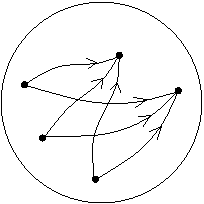
\includegraphics[width=40\unitlength]{view}}
\cell{-16}{-1}{c}{B_1}
\cell{-10}{-11}{c}{B_2}
\cell{0.5}{-18}{c}{B_3}
\cell{3}{11}{c}{A}
\cell{14.5}{4}{c}{A'}
\cell{16}{16}{c}{\cat{A}}
\end{picture}%
\caption{If $\cat{A}(B, A) \iso \cat{A}(B, A')$ naturally in $B$, then $A
  \iso A'$.}
\label{fig:view}
\end{figure}

\begin{example} 
Consider Corollary~\ref{cor:reps-unique} in the case $\cat{A} = \Grp$.
Take two groups $A$ and $A'$, and suppose someone tells us that $A$ and
$A'$ `look the same from $B$' (meaning that $\h_A(B) \iso \h_{A'}(B)$) for
all groups $B$.  Then, for instance:
% 
\begin{itemize}
\item 
$\h_A(1) \iso \h_{A'}(1)$, where $1$ is the trivial group.  But $\h_A(1) =
\Grp(1, A)$ is a one-element set, as is $\h_{A'}(1)$, no matter what $A$
and $A'$ are.  So this tells us nothing at all.

\item 
$\h_A(\integers) \iso \h_{A'}(\integers)$.  We know that $\h_A(\integers)$
is the underlying set of $A$, and similarly for $A'$.  So $A$ and $A'$
have isomorphic underlying sets.  But for all we know so far, they might
have entirely different group structures.

\item 
$\h_A(\integers/p\integers) \iso \h_{A'}(\integers/p\integers)$ for every
prime $p$, so by Example~\ref{eg:co-reps-seeing}, $A$ and $A'$ have the
same number of elements of each prime order.%
%
\index{group!order of element of}
%
\end{itemize}
% 
Each of these isomorphisms gives only partial information about the
similarity of $A$ and $A'$.  But if we know that $\h_A(B) \iso \h_{A'}(B)$
for all groups $B$, and \emph{naturally} in $B$, then $A \iso A'$.
\end{example}

\begin{example}
The category of sets is very unusual in this respect.  For any set $A$, we have
\[
A \iso \Set(1, A) = \h_A(1),
\]
so $\h_A(1) \iso \h_{A'}(1)$ implies $A \iso A'$.  In other words, two
objects of $\Set$ are the same if they look the same from the point of view
of the one-element set.  This is a familiar feature of sets: the only thing
that matters about a set is its elements!

For a general category, Corollary~\ref{cor:reps-unique} tells us that two
objects are the same if they have the same generalized%
%
\index{element!generalized}
%
elements of all shapes.  But the category of sets has a special property:
if I choose an object and tell you only what its generalized elements of
shape $1$ are, then you can deduce exactly what my object must be.
\end{example}

\begin{example} 
\label{eg:yon-adjts-unique}
Let $G\from \cat{B} \to \cat{A}$ be a functor, and suppose that both $F$
and $F'$ are left adjoint to $G$.  Then for each $A \in \cat{A}$, we have
\[
\cat{B}(F(A), B)
\iso
\cat{A}(A, G(B))
\iso 
\cat{B}(F'(A), B)
\]
naturally in $B \in \cat{B}$, so $\h^{F(A)} \iso \h^{F'(A)}$, so $F(A) \iso
F'(A)$ by Corollary~\ref{cor:reps-unique}.  In fact, this isomorphism is
natural in $A$, so that $F \iso F'$.  This shows that left adjoints are
unique, as claimed in Remark~\ref{rmks:adjts}\bref{rmks:adjts:uniqueness}.
Dually, right adjoints are unique.  See also Exercise~\ref{ex:adjts-unique}.
\end{example}

\begin{example}
Corollary~\ref{cor:reps-unique} implies that if a set-valued functor is
isomorphic to both $\h^A$ and $\h^{A'}$ then $A \iso A'$.  So the functor
\emph{determines} the representing object, if one exists.  For instance, take
the functor 
\[
\Bilin(U, V; \dashbk)\from \Vect_k \to \Set
%
\index{map!bilinear}
%
\]
of Example~\ref{eg:co-reps-tensor}.  Corollary~\ref{cor:reps-unique}
implies that up to isomorphism, there is \emph{at most one} vector space
$T$ such that
\[
\Bilin(U, V; W) \iso \Vect_k(T, W)
\]
naturally in $W$.  It can be shown that there does, in fact, exist such a
vector space $T$.  Since all such spaces $T$ are isomorphic, it is
legitimate to refer to any of them as \emph{the}%
%
\index{uniqueness}
%
tensor%
%
\index{tensor product}
%
product of $U$ and $V$.
\end{example}
%
\index{functor!representable!isomorphism of representables|)}
%

\exs


\begin{question}        
\label{ex:ff-refl-isos}
Prove Lemma~\ref{lemma:ff-refl-isos}.
\end{question}


\begin{question}
Let $\cat{A}$ be a locally small category.  Prove each of the following
statements directly (without using the Yoneda lemma).
% 
\begin{enumerate}[(b)]
\item 
$\h_\bl\from \cat{A} \to \pshf{\cat{A}}$ is faithful.

\item 
$\h_\bl$ is full.

\item
Given $A \in \cat{A}$ and a presheaf $X$ on $\cat{A}$, if $X(A)$ has an
element $u$ that is universal in the sense of Corollary~\ref{cor:rep-univ},
then $X \iso \h_A$.
\end{enumerate}
\end{question}


\begin{question}
Interpret the theory of Chapter~\ref{ch:rep} in the case where the category
$\cat{A}$ is discrete.  For example, what do presheaves look like, and
which ones are representable?  What does the Yoneda lemma tell us?  Does
its proof become any shorter?  What about the corollaries of the Yoneda
lemma?
\end{question}


\begin{question}        
\label{ex:adjts-unique}
Let $\cat{B}$ be a category and $J\from \cat{C} \to \cat{D}$ a functor.
There is an induced functor
\[
J \of \dashbk\from \ftrcat{\cat{B}}{\cat{C}} \to \ftrcat{\cat{B}}{\cat{D}}
\]
defined by composition with $J$.  
% 
\begin{enumerate}[(b)]
\item 
Show that if $J$ is full and faithful then so is $J\of\dashbk$.

\item 
Deduce that if $J$ is full and faithful and $G, G'\from \cat{B} \to
\cat{C}$ with $J \of G \iso J \of G'$ then $G \iso G'$.

\item 
Now deduce that right adjoints are unique:%
%
\index{adjunction!uniqueness of adjoints}
%
if $F\from \cat{A} \to \cat{B}$ and $G, G'\from \cat{B} \to \cat{A}$ with
$F \ladj G$ and $F \ladj G'$ then $G \iso G'$.  (Hint: the Yoneda embedding
is full and faithful.)
\end{enumerate}
\end{question}



